\chapter{Fundamental Group}

\section{Definition of $\Pi_1 (X,b)$}

\begin{definition}{Homotopic Relative}\\
Let $A \subseteq X$ be topological spaces. We say $f,g : X \rightarrow Y$ are homotopic relative to $A$ if there exists $H : X \times [0,1] \rightarrow Y$, s.t.:
$$\begin{cases}
    H(x,0) = f(x)\\
    H(x,1) = g(x)
\end{cases} \;\; and \;\;\;\;\; H(a,t) = f(a) = g(a) \;\;\forall a \in A,t\in I.$$
\end{definition}

\begin{definition}{Fundamental Group}\\
The \textit{fundamental group of topological space $X$ at base point $b \in X$} is defined by
$$\Pi_1 (X,b) := \frac{\{ l : I \rightarrow X \;\;loop\;based\;at\;b,\;i.e.:\;f(0)=f(1)=b \} } {\sim \;homotopy\;\;relative\;\;to\;\; \{0,1 \}}$$
which is also called the 1-st homotopy group.
\end{definition}

\begin{proposition}
    The fundamental group $\Pi_1 (X,b)$ has group structure.
\end{proposition}

\begin{proof}
    Denote $\{ l : I \rightarrow X \;\;loop\;based\;at\;b,\;i.e.:\;f(0)=f(1)=b \}$ by $L$.
    \begin{itemize}
        \item We need to firstly define an operation on the fundamental group $\Pi_1 (X,b)$: 
        \begin{itemize}
            \item For two loops $l,l' \in L$, define the binary operation $\cdot : L \times L \rightarrow L$ by
            $$(l \cdot l') (s) := \begin{cases}
                l(2s) &0 \leq s \leq 1/2\\
                l'(2s-1) &1/2 \leq s \leq 1
            \end{cases}.$$
            It remains to show that $l \cdot l' \in L$ by showing $(l \cdot l')(0) = l(0) =b $ and $ (l \cdot l') (1) = l'(0) = b$.
            \item Define $* : \Pi_1 (X,b) \times \Pi_1 (X,b) \rightarrow \Pi_1 (X,b)$ by
            $$[l] * [l'] := [l \cdot l'].$$
            It remains to check the well-defined-ness of $*$, i.e.: if $l_1 \simeq l_2$ and $l_1' \simeq l_2'$ relative to $\{0,1\}$, then $l_1 \cdot l_2 \simeq l_1' \cdot l_2'$ relative to $\{0,1\}$: 
            
            Take the homotopies $H$ between $l_1$ and $l_2$ and $K$ between $l_1'$ and $l_2'$. Then define $G : I \times I \rightarrow X$ by
            $$G(s,t) :=\begin{cases}
                H(2s,t) &0\leq s \leq 1/2\\
                K(2s-1,t) &1/2 \leq s \leq 1
            \end{cases}.$$
            One can check that $G(s,0) = (l_1 \cdot l_2) (s)$ and $G(s,1) = (l_1' \cdot l_2') (s)$.
            \item It remains to show that $*$ is associative: 
            
            Take $[u],[v],[w] \in \Pi_1 (X,b)$. Define $H' : I \times I \rightarrow X$ by
            $$H' (s,t) := \begin{cases}
                u(\frac{4s}{2-t}) &0 \leq s \leq \frac{1}{2} - \frac{1}{4}t\\
                v(4s-2 +t) &\frac{1}{2} - \frac{1}{4}t \leq s \leq \frac{3}{4} - \frac{1}{4}t\\
                w(4s - 3 + \frac{t}{1+t}) &\frac{3}{4} - \frac{1}{4}t \leq s \leq 1
            \end{cases}$$
            which is easy to check that $H'$ is the homotopy between $(u \cdot v) \cdot w \simeq u \cdot (v \cdot w)$. Since $u(0) = u(1) = v(0) = v(1) = w(0) = w(1) =b$, then we have
            $$([u] * [v] ) * [w] = [u] * ([v] * [w]).$$
        \end{itemize}
        \item $$e_{\Pi_1(X,b)} = [c_b]$$
        where $c_b(s) = b$ for all $s$.
        \item For each loop $l \in L$, define:
        $$l^{-1} (s) := l(1-s)$$
        for any $s \in I$. Then it remains to show that $l \cdot l^{-1} \simeq c_b$ by constructing $H''  : I \times I \rightarrow X$ as
        $$H'' (s,t) := \begin{cases}
            l(2s(1-t)) &0\leq s \leq 1/2\\
            l ((2-2s)(1-t)) &1/2 \leq s \leq 1
        \end{cases}$$
        which is the homotopy between $l \cdot l^{-1} \simeq c_b$ and that similarly for $ l^{-1} \cdot l \simeq c_b$.
    \end{itemize}
\end{proof}

\begin{definition}{Simple connectivity}\\
$X$ is simply connected if for any $b \in X$, s.t.:
$$\Pi_1 (X,b) \cong \{ e\}.$$
\end{definition}

\noindent\textbf{Example:}
\begin{itemize}
    \item $\mathbb{R}^2$ is simply connected: 
    
    Since $\mathbb{R}^2$ is convex, then we can use the linear homotopy between any loop and some point.
    \item $\mathbb{R}^2 \setminus \{0\}$ is \textbf{NOT} simply connected, since the loops who encircle $0$ can not be homotopic to any $c_b$.
\end{itemize}

\begin{proposition}
    If $b,b' \in X$ are connected by a path $\omega : [0,1] \rightarrow X$, then one has
    $$\Pi_1 (X,b) \cong \Pi_1 (X,b')$$
\end{proposition}

\begin{proof}
    Construct a map $\omega_* : \Pi_1(X,b) \rightarrow \Pi_1(X,b')$ by
    $$\omega_* [l] := [\omega^{-1} \cdot l \cdot \omega]$$
    \begin{itemize}
        \item \textit{$\omega_*$ is a group homomorphism:}
        \begin{align*}
            \omega_* ([l] \cdot [l']) &= \omega_*[l \cdot l'] := [\omega^ {-1} \cdot l \cdot l' \cdot \omega] = [\omega^ {-1} \cdot l \cdot \omega \cdot \omega^{-1} \cdot l' \cdot \omega]\\
            &= [\omega^ {-1} \cdot l \cdot \omega \cdot \omega^{-1}] \cdot [l' \cdot \omega] := \omega_*[l] \cdot \omega_*[l']
        \end{align*}
        \item \textit{$\omega_*$ is invertible:} Take $\alpha : \Pi_1 (X,b') \rightarrow \Pi_1 (X,b)$ given by
        $$\alpha [l'] := [\omega \cdot l' \cdot \omega^{-1}]$$
        Then check that $\alpha \cdot \omega_* =id$ and $ \omega_* \cdot \alpha = id$, i.e.: $\alpha = \omega_*^{-1}$.
    \end{itemize}
    Therefore, $\omega_*$ is a group isomorphism.
\end{proof}

\noindent\textbf{Remark:} If $X$ is \textit{path-connected}, then for any $x_1,x_2 \in X$, one has
$$\Pi_1 (X, x_1) \cong \Pi_1 (X,x_2)$$
Moreover, in such case, we'll write $\Pi_1(X)$ instead of $\Pi_1 (X,b)$. But when computing, we need to pick a based point.

\begin{definition}{Induced Homomorphism}\\
Let $(X,x_0)$ and $(Y,y_0)$ be two topological spaces with basepoint $x_0$ and $y_0$, respectively, and let $f : X \rightarrow Y$ be a continuous map with $f(x_0) = y_0$. Then every loop $l : I\rightarrow X$ based at $x_0$ gives a loop $f \circ l: I \rightarrow Y$, i.e.: $f$ induces a group homomorphism $f_*: \Pi_1 (X,x_0) \rightarrow \Pi_1 (Y, y_0)$ satisying
$$f_* [l] := [f \circ l]$$
\end{definition}

\noindent\textbf{Check:} $f_*$ is well-defined: If $l \simeq l'$ relative to $\{ 0,1 \}$ based at $x_0$, then there exists a homotopy $H : I \times I \rightarrow X$, s.t.: for any $t \in I$,
\begin{align*}
    &H(t,0) =l(t), H(t,1)=l'(t)\\
    &H(a,t) = l(a) = l'(a) =x_0, \;\forall a \in \{0,1\}
\end{align*}
Then consider $K: I \times I \overset{H}{\rightarrow} X \overset{f}{\rightarrow} Y$, i.e.:
$$K = f \circ H$$
Then one has
\begin{align*}
    &K(t,0) := f(H(t,0)) = f(l(t)) = (f \circ l) (t)\\
    &K(t,1) := f(H(t,1)) = f(l'(t)) = (f \circ l') (t)\\
    &K(a,t) := f(H(a,t)) =(f \circ l)(a) = (f \circ l')(a),\; \forall a\in \{0,1\}
\end{align*}
Hence, $f \circ l \simeq f \circ l'$ relative to $\{0,1\}$ based at $x_0$.

\begin{proposition}
    \begin{enumerate}
        \item $(id_X)_* = id_{\Pi_1(X,x_0)}$
        \item $(g \circ f)_* = g_* \circ f_*$
        \item If $f \simeq f'$ relative to $x_0 \in X$, then $f_* = (f')_*$
    \end{enumerate}
\end{proposition}

\begin{corollary}
    Let $X,Y$ be path-connected and let $X \simeq Y$. Then one has
    $$\Pi_1 (X) \cong \Pi_1(Y)$$
\end{corollary}

\begin{proof}
    Since $X \simeq Y$, then by def, there exist continuous functions $f,g$, s.t.:
    \begin{align*}
        &X \overset{f}{\rightarrow} Y \overset{g}{\rightarrow} X \simeq id_X\\
        &Y \overset{g}{\rightarrow} X \overset{f}{\rightarrow} Y \simeq id_Y
    \end{align*}
    \noindent\textit{WARNING:} We can NOT use $(g \circ f)_* = (id_X)_*$, since $g \circ f \simeq id_X$ is not relative to $x_0$.

    Denote $(g \circ f)(x_0)$ by $x_1$. By the hypothesis of corollary, there exists a path $\omega: I \rightarrow X$ from $x_0$ to $x_1$. Then consider $H: X \times I \rightarrow X$ to be the homotopy between $g \circ f \simeq id_X$ given by
    $$H(x_0 ,t) := \omega(t)$$
    and the induced group homomorphism is 
    $$\Pi_1 (X,x_0) \overset{f_*}{\rightarrow} \Pi_1 (Y, y_0) \overset{g_*}{\rightarrow} \Pi_1 (X,x_1)$$
    For any loop $l$ based at $x_0$, consider $K: I\times I \overset{l \times id}{\rightarrow} X \times I \overset{H}{\rightarrow} X$, i.e.:
    $$K (t,s) := H(l(t),s)$$
    Then $K$ gives the homotopy between $g \circ f \circ l$ and $l$. Note that $[\omega^{-1} (g \circ f \circ l)\omega] = [l]$. Then by the def of $\omega_*$ in proposition 8.5, one has
    $$[l] = \omega_* [g \circ f \circ l] = \omega_* \circ g_* \circ f_* [l]$$
    Hence $\omega_* \circ g_* \circ f_* = id_{\Pi_1(X,x_0)}$. Since $\omega_*$ is an group isomorphism which is proved in proposition 8.5, then we have: $g_*$ is surjective and $f_*$ is injective. Similarly, $g_*$ is injective and $f_*$ is injective. Then we're done.
\end{proof}

\section{Computation of $\Pi_1 (X,b)$}

\begin{definition}
    Let $K = (X,\Sigma)$ be a simplicial complex and let $\alpha := (v_0,v_1, \cdots, v_n)$ and $\beta:= (w_0 ,w_1,\cdots, w_m)$ be two edge paths.
    \begin{itemize}
        \item \textbf{Edge Loop:} $\alpha$ is an edge loop based at $v_0$ if $v_n = v_0$
        \item \textbf{Concatenation:} If $v_n= w_0 =w_m =v_0$, then we define the \textit{concatenation of loops based at $v_0$} by
        $$\alpha \cdot \beta = (v_0,\cdots, v_n=v_0) \cdot (w_0 = v_0 ,\cdots, w_m=v_0) := (v_0 , \cdots, v_n,w_1, \cdots ,w_m)$$
    \end{itemize}
\end{definition}

\begin{definition}{Elementary Contraction/Expansion}\\
Let $\alpha,\beta$ be edge paths.
\begin{itemize}
    \item An \textit{elementary contraction} of $\alpha$ is given by one of the 3 operations below:
    \begin{enumerate}
        \item replacing $\cdots v_{i-1}v_i \cdots$ by $\cdots v_{i-1} \cdots$ if $v_{i-1} = v_i$;
        \item replacing $\cdots v_{i-1}v_iv_{i+1} \cdots$ by $\cdots v_{i-1}  \cdots$ if $v_{i-1} = v_{i+1}$;
        \item replacing $\cdots v_{i-1}v_iv_{i+1} \cdots$ by $\cdots v_{i-1} v_{i+1} \cdots$ if $\{ v_{i-1},v_{i}, v_{i+1} \} \in \Sigma$.
    \end{enumerate}
    \item An \textit{elementary expansion} is the reverse of an elementary contraction.
    \item $\alpha$ and $\beta$ are \textit{equivalent}, denoted as $\alpha \sim \beta$, if they differ by a finite number of elementary contractions or expansions.
\end{itemize}
\end{definition}

\noindent\textbf{Example:} Let $K = (V,\Sigma)$ where $V = \{ 1,2,3\}$ and $\Sigma= \{ \{1\} ,\{2\} ,\{3\}, \{1,2\}, \{2,3\} ,\{1,3\} \}$.
\begin{align*}
    11123213211231 \sim 12321321231 \sim 1323231 \sim 13231 \sim 131 \sim 1
\end{align*}

\noindent\textbf{Remark:} If $\alpha \sim \beta$, then the topological realization of $\alpha$ and $\beta$ are homotopic.

\begin{definition}{Edge Loop Group}\\
Let $K= (V, \Sigma)$ and $b \in V$. The \textit{edge loop group based at $b$} is defined by
$$\Pi_1(K,b) := \frac{\{edge\;\;loops\;\;based\;\;at\;\;b \}}{\sim\; elementary\;\;contractions\;\;or\;\; expansions}$$
\end{definition}

\begin{proposition}
    $(\Pi_1 (K,b) , *)$ has a group structure where
    $$[\alpha] * [\beta] := [\alpha \cdot \beta]$$
\end{proposition}

\begin{proof}
    \begin{itemize}
        \item \textit{Well-defined-ness of $*$:} If $\alpha \sim \alpha'$ and $\beta \sim \beta'$, i.e.: $[\alpha] = [\alpha']$ and $[\beta] = [\beta']$, then $[\alpha] * [\beta] = [\alpha'] * [\beta']$.
        \item \textit{Associativity of $*$:} Clearly.
        \item \textit{Identity:} $e = [b]$, by operation 1.
        \item \textit{Inverse:} $[b v_1 \cdots v_{n-1} b]^{-1} = [bv_{n-1} \cdots v_1b]$, by operation 2.
    \end{itemize}
\end{proof}

\begin{proposition}
    Let $K = (V, \Sigma)$ where $V = \{1,2,3\}$ and $\Sigma =\{ \{1\},\{2 \},\{3\} ,\{1,2\}, \{1,3\}, \{2,3\} \}$. Then
    $$\Pi_1 (K) \cong (\mathbb{Z},+)$$
\end{proposition}

\begin{proof}
    \textbf{Intuition:} Since $\{ 1,2,3\} \not \in \Sigma$, then we can NOT apply operation 3, i.e.: $[\cdots (123)^{m_1} \cdots] \neq [\cdots (123)^{m_2} \cdots]$ if $m_1\neq m_2$.

    Define the \textit{winding number of $\alpha$}, $\Phi:\{$edge loops based at 1$\} \rightarrow \mathbb{Z}$, by
    $$\Phi(\alpha) := \# \{23\;\;appearing\;\;in\;\;\alpha \}- \#\{ 32\;\; appearing\;\;in\;\;\alpha \}$$
    and then define a map $\phi : \Pi_1 (K,1) \rightarrow \mathbb{Z}$ by
    $$\phi[\alpha] := \Phi(\alpha)$$
    \begin{itemize}
        \item \textit{$\phi$ is a group homomorphism:} 
        \begin{align*}
            \phi ([\alpha] * [\beta])  &= \phi[\alpha \cdot \beta] =\Phi (\alpha \cdot \beta)\\
            &= \# \{23\;\;appearing\;\;in\;\;\alpha \cdot \beta \}- \#\{ 32\;\; appearing\;\;in\;\;\alpha \cdot \beta \}\\
            &=\# \{23\;\;appearing\;\;in\;\;\alpha \} +\# \{23\;\;appearing\;\;in\;\;\beta \}- \#\{ 32\;\; appearing\;\;in\;\;\alpha \}- \#\{ 32\;\; appearing\;\;in\;\;\beta\}\\
            &= \# \{23\;\;appearing\;\;in\;\;\alpha \} - \#\{ 32\;\; appearing\;\;in\;\;\alpha \} + \# \{23\;\;appearing\;\;in\;\;\beta \}- \#\{ 32\;\; appearing\;\;in\;\;\beta\}\\
            &= \Phi(\alpha) + \Phi(\beta) = \phi [\alpha] + \phi [\beta]
        \end{align*}
        \item \textit{$\phi$ is surjective:} For any $n \in \mathbb{Z}$,
        $$\begin{cases}
            n>0 \Rightarrow \phi ((123)^n1) =n\\
            n=0 \Rightarrow \phi(1) =n\\
            n<0 \Rightarrow \phi((132)^n1) =n
        \end{cases}$$
        \item \textit{$\phi$ is injective:} 
        \begin{align*}
            \ker \phi &:= \{ 0\} = \{ [\beta] \mid \# \{23\;\;appearing\;\;in\;\;\alpha \} = \#\{ 32\;\; appearing\;\;in\;\;\alpha \} \}\\
            &= \{ [1]\} 
        \end{align*}
    \end{itemize}
    Therefore, $\phi$ is a group isomorphism, i.e.:
    $$\Pi_1 (K) = \Pi_1(K,1) \cong \mathbb{Z}$$
\end{proof}

\noindent\textbf{Remark:} $\Pi_1 (K)$ is infinite cyclic.

\begin{theorem}
    $$\Pi_1(K,b) \cong \Pi_1 (|K|,b)$$
    where $\Pi_1(K,b)$ denotes the edge loop group and $\Pi_1 (|K|,b)$ denotes the fundamental group.
\end{theorem}

\noindent\textbf{Recall:} Simplicial Approximation Theorem: for any $f :I \rightarrow |K|$, there is a simplicial complex (subdivision) of $I$
$$I_n := \{ [0, \frac{1}{n}] , \cdots, [\frac{n-1}{n},1]\}$$
so that $V_{I_n} = \{0, \frac{1}{n} ,\cdots, \frac{n-1}{n},1\}$, $ \Sigma  _{I_n} =\{ \{0, \frac{1}{n}\} , \cdots, \{\frac{n-1}{n},1\} \}$ and $|I_n| \cong I$ are homeomorphic. Then take a simpicial map $g: I_n \rightarrow K$, s.t.:
$$|g| \simeq f$$
relative to "overlapping part", e.g.:
\begin{figure}[htbp]
    \centering
    \begin{tikzpicture}[scale=1.5, thick]
        \colorlet{penred}{red!80!black}
        \colorlet{penblue}{blue!80!black}
    
        \coordinate (P1) at (0, 0);
        \coordinate (P2) at (1, 2);
        \coordinate (P3) at (2, 0.5);
        \coordinate (P4) at (3, 2);
        \coordinate (P5) at (4, 0.5);
        \coordinate (P6) at (5, 1.5);
    
        \draw[thin] (2.2, 0.5) -- (2.55, 1.4);
        \draw[thin] (2.6, 0.5) -- (2.95, 1.4);
        \draw[thin] (3.1, 0.5) -- (3.45, 1.3);
        \draw[thin] (3.6, 0.5) -- (3.8, 0.8);
    
        \draw[very thick] (P1) -- (P2) -- (P3) -- (P4) -- (P5) -- (P6);
        \draw[very thick] (P3) -- (P5); 
    
        \draw[penred, thick]
            (-0.05, 0.1) --
            (1, 2.15) --
            (2, 0.65) --
            (3, 2.15) --
            (4, 0.65) --
            (4.95, 1.6);
    
        \draw[penblue, thick]
            (0.05, -0.1) --
            (1, 1.85) --
            (1.95, 0.35);
    
        \draw[penblue, thick]
            (1.95, 0.35)
            .. controls (2.3, 0.9) and (2.6, 0.6) .. (2.9, 0.7)
            .. controls (3.2, 0.8) and (3.6, 0.5) ..
            (4.05, 0.35);
    
        
        \draw[penblue, thick]
            (4.05, 0.35) --
            (5.05, 1.4);
    
        
        \node at (-0.2, -0.2) {$1$};
        \node at (0.8, 2.2) {$2$};
        \node at (1.8, 0.2) {$3$};
        \node at (3, 2.3) {$4$};
        \node at (4.2, 0.2) {$5$};
        \node at (5.2, 1.5) {$6$};
    
        
        \node[penblue] (omega) at (3.1, -0.1) {$\omega$};
        \draw[penblue, thin] (omega) -- (3.25, 0.65);
    
        
        \node[penred, right] at (5.5, 1.8) {\Large $|g|: 1 \to 2 \to 3 \to 4 \to 5 \to 6$};
        \node[penblue, right] at (5.5, 0.8) {\Large $f: 1 \to 2 \to 3 \xrightarrow{\omega} 5 \to 6$};
        
    \end{tikzpicture}
    \caption{Paths of mappings $|g|$ and $f$}
\end{figure}
where the "overlapping part" of $|g|$ and $f$ are $1 \to 2 \to 3$ and $5 \to 6$.

\begin{proof}
    (\textit{of Theorem 8.14})
    For any edge loop $\alpha$, define the realization of $\alpha$, $g_\alpha: I \to \Pi_1 (|K|,b)$. Then define $\Theta: \Pi_1 (K,b) \to \Pi_1 (|K|,b)$ by
        $$\Theta [\alpha] := [g_\alpha]$$
    The well-defined-ness of $\Theta$ is easy to check, since if $\alpha \sim \beta$, then $g_\alpha \sim g_\beta$. Then for two edge loops $\alpha_1$ and $\alpha_2$, 
    $$\Theta [\alpha_1] \cdot \Theta [\alpha_2] = [g_{\alpha_1}] \cdot [g_{\alpha_2}] = [g_{\alpha_1} \cdot g_{\alpha_2}] \overset{(*)}{=}[g_{\alpha_1 \alpha_2}] = \Theta ([\alpha] \cdot [\beta])$$
    where $(*)$ holds since $[g_{\alpha_1} \cdot g_{\alpha_2}]$ and $[g_{\alpha_1 \alpha_2}]$ have the same path with the different speeds, which follows that $\Theta$ is a group homomorphism.

    Now it remains to show that $\Theta$ is an group isomorphism:
    \begin{itemize}
        \item \textit{$\Theta$ is surjective:} Take a loop $f:I \to |K|$ based at $b$, by Simplicial Approximation Theorem, take $I_n$ to be in \textbf{Recall}, i.e.: $I_n \cong I$. Then there exists a simplicial map $g: I_n \to K$, s.t.:
        $$|g| \simeq f$$
        Now take $\alpha := (b=g(0), g(1/n), \cdots ,g((n-1)/n), g(1) =b)$, which is an edge loop in $K$ based at $b$, since for any $i \in \{ 0,\cdots,n\}$, $g(i/n)$ is either a vertice in $K$ or a point on one of the edges in $K$, with $|g| = g_\alpha : I \to |K|$. Hence, $[g_\alpha] = [f] \in \Pi_1 (|K|,b)$.
        \item \textit{$\Theta$ is injective:} For any edge loop $\alpha$ based at $b$ such that $[\alpha] \in \ker \Theta$, i.e.: $\Theta [\alpha] := [g_\alpha] = e_{\Pi_1 (|K|,b)}$, i.e.:
        $$g _ \alpha \simeq c_b$$
        Hence, there exists a homotopy $H:I \times I \to |K|$ between $g_\alpha$ and $c_b$. Then apply Simplicial Approximation Theorem on $H$. Namely, there exists a sufficiently large positive integer $r$, s.t.: $(I \times I)_r$ is a subdivision of $I \times I$ with $r \times r$ squares (every square contains two 2-simplices), i.e.:
        $$|(I \times I)_r| \cong I \times I$$
        and a simplicial map $G : (I \times I)_r \to K$, s.t.: $|G| \simeq H$, as figure 8.2 shown.
        \begin{figure}[htbp]
            \centering
            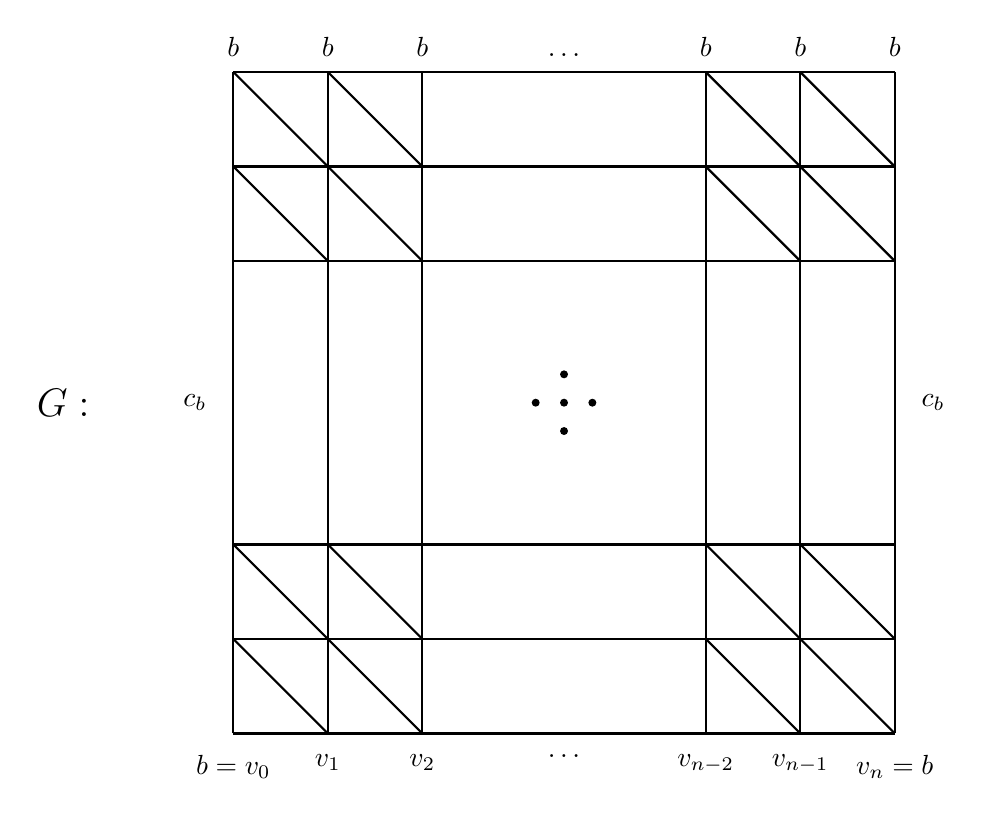
\begin{tikzpicture}[scale=1.2, thick]
        
        
                \foreach \y in {0, 1, 2, 5, 6, 7} {
                    \draw (0,\y) -- (7,\y);
                }
        
       
                \foreach \x in {0, 1, 2, 5, 6, 7} {
                    \draw (\x,0) -- (\x,7);
                }

        
                \foreach \x in {0, 1, 5, 6} {
                    \foreach \y in {0, 1, 5, 6} {
                        \draw (\x, \y+1) -- (\x+1, \y);
                    }
                }

        
                \node[above=2pt] at (0,7) {$b$};
                \node[above=2pt] at (1,7) {$b$};
                \node[above=2pt] at (2,7) {$b$};
                \node[above=2pt] at (3.5,7) {$\dots$};
                \node[above=2pt] at (5,7) {$b$};
                \node[above=2pt] at (6,7) {$b$};
                \node[above=2pt] at (7,7) {$b$};

        
                \node[below=4pt] at (0,0) {$b=v_0$};
                \node[below=4pt] at (1,0) {$v_1$};
                \node[below=4pt] at (2,0) {$v_2$};
                \node[below=4pt] at (3.5,0) {$\dots$};
                \node[below=4pt] at (5,0) {$v_{n-2}$};
                \node[below=4pt] at (6,0) {$v_{n-1}$};
                \node[below=4pt] at (7,0) {$v_n=b$};

        
                \node[left=6pt] at (0,3.5) {$c_b$};
                \node[right=6pt] at (7,3.5) {$c_b$};

        
                \node at (-1.8, 3.5) {\Large $G:$};

        
                \fill (3.5, 3.5) circle (1.2pt);
                \fill (3.5, 3.8) circle (1.2pt);
                \fill (3.5, 3.2) circle (1.2pt);
                \fill (3.2, 3.5) circle (1.2pt);
                \fill (3.8, 3.5) circle (1.2pt);

            \end{tikzpicture}
            \caption{}
        \end{figure}

        where $\alpha = (b=v_0, v_1 ,\cdots, v_{n-1}, v_n =b)$.
        Hence, one has
        $$\alpha = bv_1 \cdots v_{n-1}b \sim \cdots \sim bb \cdots bb \sim b$$
        which is equivalent to $[\alpha] = [b]$, which is the trivial edge loop class in $\Pi_1 (|K|,b)$, i.e.:
        $$\ker \Theta = \{[b]\} = \{e_{\Pi_1 (|K|,b)} \}$$
        which implies the injectivity of $\Theta$.
    \end{itemize}
\end{proof}

\begin{corollary}
    $$\Pi_1 (|K|) \cong (\mathbb{Z},+)$$
    where $K$ is the simplicial complex defined in proposition 8.13.
\end{corollary}

\begin{definition}{Skelecton}\\
Let $K = (V, \Sigma)$ be a simplicial complex. The \textit{n-skelecton} of $K$ is the simplicial complex $K^{(n)} = (V^{(n)} , \Sigma^{(n)})$ where 
$$V^{(n)} := V\;\;and\;\; \Sigma^{(n)} := \{ \sigma \in \Sigma \mid |\sigma| \leq n+1 \}$$
\end{definition}

\begin{corollary}
    For $n \geq 2$,
    $$\Pi_1 (|K|, b) \cong \Pi_1 (|K^{(n)}|,b)$$
\end{corollary}

\begin{proof}
    Using edge loops, some elementary contraction/expansion on edge loops involve only information on 2-simplex in.
\end{proof}

\noindent\textbf{Remark:} If $n=1$, then we only have the information on edges, but we threw away all the faces. Hence, we can NOT use \textit{operation 3}. Here we imply the difference between proposition 8.13 above and proposition 8.18 below.

\begin{proposition}
    Let $K = (V, \Sigma)$ where $V = \{1,2,3\}$ and $\Sigma =\{ \{1\},\{2 \},\{3\} ,\{1,2\}, \{1,3\}, \{2,3\}, \{1,2,3\} \}$. Then $K$ is simply-connected.
\end{proposition}

\begin{proof}
    It's equivalent to show that $\Pi_1 (K,1) = \{ e\} = \{ [1]\}$. For any edge loop $\alpha = (1=v_0, v_1, \cdots, v_{n-1} , v_n=1)$ based at $1$, by operation 1, we can take $\{v_{i_1} ,\cdots, v_{i_k} \} \subseteq \{ v_1 ,\cdots, v_{n-1} \}$ to be such that $v_{i_1} \neq 1$, $v_{i_k} \neq 1$, $v_{i_j} \neq v_{i_{j+1}}$ for any $j$, and
    $$[\alpha] = [1 v_{i_1} \cdots v_{i_k}1]$$
    WLOG, let $v_{i_1} =2$. Then $[\alpha] = [123 \cdots]$ or $[121 \cdots]$. Hence, if $[\alpha] = [123 \cdots]$, then by operation 3, $[\alpha] = [13 \cdots]$ and if $[\alpha] = [121 \cdots]$, then by operation 2, $[\alpha] = [1 \cdots]$. Repeat this procedure, and then we can get $[\alpha] = [1]$. Then we're done.
\end{proof}

\begin{proposition}
    For any $n \geq 2$, 
    $$\Pi_1 (\mathbb{S}^n) \cong \{e\}$$
\end{proposition}

\begin{proof}
    Consider the simplicial complex $K= (V,\Sigma)$ given by the boundary of the simplicial complex generated by $V= \{ 1,\cdots, n+1\}$. Then one has
    $$\mathbb{S}^n = |K|$$
    Hence, by theorem 8.14 $(*)$ and corollary 8.17 $(**)$,
    \begin{equation*}
        \Pi_1 (\mathbb{S}^n) = \Pi_1({|K|}) \overset{(*)}{\cong} \Pi_1 (K) \overset{(**)}{\cong} \Pi_1 (|K^{(2)}|) \tag{\#}
    \end{equation*}
    For any edge loop $\alpha = (1= v_0, v_1 ,\cdots, v_{n-1}, v_n=1)$ based at $1$, after using operation 1 and 2, we can get $\alpha \sim (1= v_{i_0}, v_{i_1}, \cdots, v_{i_{k-1}}, v_{i_k}=1)$. Then for any $j \in \{1, \cdots ,k-1\}$, $\{ v_{i_{j-1}}, v_{i_{j}}, v_{i_{j+1}} \}$ forms a face of $K^{(2)}$. Hence, after using operation 3, we can finally get $[\alpha] = [1] \in \Pi_1 (|K^{(2)}|,1)$. Therefore,
    $$\Pi_1 (|K^{(2)}|,1) \cong \{ [1]\} \cong \{ e\}.$$
\end{proof}

\begin{theorem}{Browwer's Fixed Point Theorem}\\
For any $n \in \mathbb{N}_+$, let $\mathbb{D}^n$ be the n-dim'l disk, i.e.:
$$\mathbb{D}^n := \{ x \in \mathbb{R}^n \mid ||x||\leq 1 \}$$
For any continuous map $f: \mathbb{D}^n \to \mathbb{D}^n$, there exists a fixed point, i.e.: there exists $x_0 \in \mathbb{D}^n$, s.t.:
$$f(x_0) = x_0$$
\end{theorem}

\begin{proof}
    Suppose on the contrary that there is a cont map $f : \mathbb{D}^n \to \mathbb{D}^n$ s.t.: for any $x \in \mathbb{D}^n$, $f(x) \neq x$. Then we can construct a ray pointing from $f(x)$ to $x$ uniquely, denoted as $l_x$. Hence, there exists a point $p_x$, s.t.:
    $$\{p_x\} = l_x \cap \partial \mathbb{D}^n = l_x \cap \mathbb{S}^{n-1}$$
    Then we can construct a map $\overline{f}: \mathbb{D}^n \to \mathbb{S}^{n-1}$ by
    $$\overline{f} (x) := p_x$$
    \begin{itemize}
        \item \textbf{Claim:} $\overline{f}$ is a retraction from $\mathbb{D}^n$ onto $\mathbb{S}^{n-1}$.
        \begin{proof}
        Let $i: \mathbb{S}^{n-1} \to \mathbb{D}^n$ be the inclusion map.
            \begin{itemize}
                \item \textit{$\overline{f}$ is continuous:} Since $f$ is cont and $f(x) \neq x$ for all $x \in \mathbb{D}^n$, then the change in the direction of the rays is cont and hence $\overline{f}$ is cont.
                \item \textit{$\overline{f} \circ i = id_{\mathbb{S}^{n-1}}$:} By def of $\overline{f}$, for any $x \in \mathbb{S}^{n-1}$
                $$(\overline{f} \circ i) (x) = \overline{f}(i(x)) = \overline{f} (x) = x = id_{\mathbb{S}^{n-1}} (x) \Rightarrow \overline{f} \circ i = id_{\mathbb{S}^{n-1}}$$
                \item \textit{$i \circ \overline{f} \simeq id_{\mathbb{D}^n}$:} Consider $H: \mathbb{D}^n \times I \to \mathbb{S}^{n-1}$ given by
                $$H(x,t) := (1-t) p_x + tx$$
                Then one has $H(x,0) = p_x = (i \circ \overline{f} )(x)$, $H(x,1) = x = id_{\mathbb{D}^n}(x)$. Hence, $H$ gives a homotopy between $i \circ \overline{f}$ and $id_{\mathbb{D}^n}$.
            \end{itemize}
            By \textit{claim}, $\Pi_1 (\mathbb{D}^2) \cong \Pi_1 (\mathbb{S}^1)$. But $\Pi_1 (\mathbb{D}^2) \cong \{ 0\}$, $\Pi_1 (\mathbb{S}^1) \cong \mathbb{Z}$, contradiction since $\{0\}$ is trivial and $\mathbb{Z}$ is NOT.
        \end{proof}
    \end{itemize}
\end{proof}

\begin{theorem}
Every non-constant polynomial $p(x) \in \mathbb{C}[x]$ has a root in $\mathbb{C}$.
\end{theorem}

\begin{proof}
    Suppose on the contrary that there exists a non-constant polynomial $p(x) \in \mathbb{C}[x]$ having NO root in $\mathbb{C}$. Then for any $x \in \mathbb{C}$, $p(x) \neq 0$, i.e.: $p: \mathbb{C} \to \mathbb{C} \setminus \{0\}$ is a map given by $p(x) := a_n x^n + \cdots + a_1 x + a_0$. For $r>0$, consider
    \begin{equation*}
    \begin{tikzcd}[row sep=large, column sep=large]
        C_r \arrow[r, hook, "i"] \arrow[dr, "p|_{C_r}"'] & \mathbb{C} \arrow[d, "p"] \\
        & \mathbb{C} \setminus \{0\}
    \end{tikzcd}
    \end{equation*}
    where $C_r:= \{ re^{i\theta} \mid 0 \leq \theta <2\pi\}$ denotes the circle in complex plane of radius $r$, i.e.: $\left. p \right|_{C_r} = p \circ i$.Then we have a diagram of group homomorphisms: 
    \begin{equation*}
    \begin{tikzcd}[column sep=large, row sep=large]
    \mathbb{Z} \cong \Pi_1(C_r) \arrow[r, "i_*"] \arrow[dr, "(p|_{C_r})_*"'] & \Pi_1(\mathbb{C}) \cong \{0\} \arrow[d, "p_*"] \\
    & \Pi_1(\mathbb{C}\setminus\{0\}) \cong \Pi_1(S^1) \cong \mathbb{Z}
    \end{tikzcd}
    \end{equation*}

    Hence, for any $m \in \mathbb{Z} \cong \Pi_1 (C_r)$,
    \begin{equation*}
        (p|_{C_r})_* (m) = (p_* \circ i_*) (m) = p_*(i_*(m)) \overset{\Pi_1 (\mathbb{C}) \cong \{0\}}{=} p_*(0) = e_{\Pi_1({\mathbb{C} \setminus \{0\}} )} \tag{\#}
    \end{equation*}
    \begin{itemize}
        \item \textbf{Claim 1:} For large $r$, we have
        $$p|_{C_r} \simeq q: C_r \to \mathbb{C} \setminus \{0\} \;\;with\;\;q(z) := \frac{p(r)}{r^n} z^n$$
        \begin{proof}
            Define $H: C_r \times I \to \mathbb{C} \setminus \{0\}$ by
            $$H(z,t) := (1-t) p(z) + q(z)$$
            \begin{itemize}
                \item \textbf{Check} that $H$ is well-defined, i.e.: $H (z,t) \neq 0$ for all $z \in C_r$, $t\in I$: Suppose on the contrary that $H( z,t) =0$ for some $z \in C_r$, $t \in I$. Then by the def of $H$ and $q$, one has $(1-t) (a_n z^n + \cdots + a_1z + a_0) = -t (\frac{p(r)}{r^n} \cdot z^n)$ and hence
                \begin{align*}
                    a_n z^n + \cdots + a_1z +a_0&= t \begin{pmatrix}
                        a_n z^n + \cdots a_1z+ a_0 - \frac{p(r)}{r^n} \cdot z^n
                    \end{pmatrix}\\
                    &= t \begin{pmatrix}
                        a_n z^n + \cdots a_1z+ a_0 - a_n z^n - \frac{a_{n-1}}{r}z^n - \cdots - \frac{a_{1}}{r^{n-1}} z^n - \frac{a_0}{r^n} z^n
                    \end{pmatrix}\\
                    &= t \begin{pmatrix}
                        a_{n-1} z^{n-1} + \cdots a_1z+ a_0 - (\frac{a_{n-1}}{r} + \cdots + \frac{a_{1}}{r^{n-1}} + \frac{a_0}{r^n} )z^n
                    \end{pmatrix}
                \end{align*}
                For large $r$, the coefficient of $z^n$ on the right hand side is nearly $0$ but the coefficient of $z^n$ on the left hand side is $a_n \not \approx 0$, contradiction.
                \item It's easy to check that $H$ gives a homotopy between $p|_{C_r}$ and $q$.
            \end{itemize}
        \end{proof}
    \end{itemize}
    Therefore, by \textit{claim 1}, for large $r$, one has
    $$(p|_{C_r})_* = q_* : \Pi_1 (C_r) \cong \mathbb{Z} \to \Pi_1 (\mathbb{C} \setminus \{ 0\}) \cong \mathbb{Z}$$
    \begin{itemize}
        \item \textbf{Claim 2:} $q_* (m) = n \cdot m$
        \begin{proof}
            Take $1 = [l] \in \Pi_1 (C_r) \cong \mathbb{Z}$ with $l (t) = re^{2\pi it}$ and $q_*(1) := [q \circ l] (1)$. Since
            $$(q \circ l) (t) = q(r e^{2\pi it}) := \frac{p(r)}{r^n} \cdot (r e^{2\pi it})^n = p(r) \cdot e^{2\pi int}$$
            then $q_*(1) = n$.
        \end{proof}
    \end{itemize}
    Contradict $(\#)$.
\end{proof}

\section{Fundamental Group of Graph}

\begin{theorem}
    Let $\Gamma = (V,E)$ be a connected graph with $|V|,|E| < \infty$. Then
    $$\Pi_1 (|\Gamma|) \cong \langle \{ e \mid e \in E \setminus E_T,\forall maximal\;tree\;T\; of \;\Gamma \} \rangle$$
    i.e.: $\Pi_1 (|\Gamma|)$ is isomorphic to free group generated by $e \in E \setminus E_T$ for all maximal tree $T$ of $\Gamma$.
\end{theorem}

\begin{corollary}
    Let $\Gamma= (V,E)$ be a connected graph with $|V| , |E| < \infty$. Then
    $$\Pi_1 (| \Gamma|) \cong \langle a_1 ,\cdots, a_n \rangle$$
    where $n=|E| - |V|+1$.
\end{corollary}

\noindent\textbf{Fact:} Planar graph: $\chi (|\Gamma|) =2$ where
$$\chi := |V| - |E| + |F|$$
(for $\Gamma$, $|F| = 0$).

